\chapter{基因组稳定性：DNA 损伤、修复与重组}\label{ch:b3:dna-repair}

海滩上的一个下午，便会使每个受阳光照射的皮肤细胞的 DNA 中出现约十万处化学\omterm{def:b3:dna-repair:lesions}{损伤}：
相邻胸腺嘧啶被紫外线焊接成二聚体、
碱基被氧化、
链被切断。即使完全没有阳光，细胞内温热的水
每天都会使约一万个嘌呤从其糖上脱落，
并把数百个胞嘧啶转变为尿嘧啶。然而，人类细胞的突变率
约为每次分裂中每百亿个碱基对出现一处改变，
——即六十亿碱基对的基因组中，每次分裂的新突变不足一个。
基因组所遭受的\omterm{def:b3:dna-repair:lesions}{损伤}与其保留的\omterm{def:b3:dna-repair:lesions}{损伤}之间的差距，
由修复来弥合：十余种酶系统沿双螺旋巡查，
识别不应存在之物，将其切除，
再以未受损的链为模板重建；两条链都断裂时，
则将其重新连接，或从姐妹染色单体上复制缺失的片段。
缺少其中任一系统的儿童——
一见阳光便灼伤，或三十多岁时罹患结肠癌——
这些情况说明了这些系统的价值。本章讨论\omterm{def:b3:dna-repair:lesions}{损伤}、修复途径、
修复最严重断裂的重组机制，减数分裂也借用这一机制，
以及修复失败时细胞的抉择：
停止分裂，还是走向死亡。

\section{DNA 出了什么问题}

\begin{definition}[DNA 损伤]\label{def:b3:dna-repair:lesions}
\index{DNA 损伤}\index{脱嘌呤}\index{脱氨基}\index{嘧啶二聚体}\index{双链断裂}\index{8-氧代鸟嘌呤}
\emph{损伤}是指 DNA 中任何使四种正常碱基偏离
正确配对、骨架完整的化学改变。自发损伤
源于水与氧的化学作用：\emph{脱嘌呤}，
即嘌呤与其糖之间的键水解，留下一个
无碱基位点（每个细胞每天约 $10^{4}$ 个）；\emph{脱氨基}，
使胞嘧啶变为尿嘧啶、5-甲基胞嘧啶变为胸腺嘧啶，以及
腺嘌呤变为次黄嘌呤（每天数百个）；\emph{氧化}，
由活性氧作用，主要生成 \emph{8-氧代鸟嘌呤}，它
与腺嘌呤配对的倾向与胞嘧啶相当；以及\emph{复制
错误}，即错掺或滑移的碱基。环境损伤
包括\emph{环丁烷嘧啶二聚体}以及 6-4
光产物，由紫外线在相邻两个
嘧啶之间形成；烷化剂产生的烷化碱基（O$^{6}$-甲基-
鸟嘌呤与胸腺嘧啶配对）；芳香烃和黄曲霉毒素产生的大体积加合物；
顺铂和氮芥产生的链间交联；
以及由电离辐射产生的单链和\emph{双链断裂}，
每细胞每戈瑞约 \num{1000} 个单链断裂和
\numrange{30}{40} 个双链断裂。
\end{definition}

\begin{proposition}[保真度阶梯]\label{prop:b3:dna-repair:fidelity}
\index{保真度}\index{校对}\index{错配修复}
复制的错误率约为每碱基对 $10^{-10}$，
分三个相乘的步骤实现。聚合酶的碱基选择依据几何构型与氢键，
出错约为每 $10^{5}$ 次一次；
由聚合酶的 3$'\to$5$'$ 外切核酸酶执行的\emph{\omterm{prop:b3:dna-repair:fidelity}{校对}}，它在延伸之前
切除延伸前错配的末端碱基，去除
\qty{99}{\%} 的此类错误；\emph{\omterm{prop:b3:dna-repair:fidelity}{错配修复}}，在复制叉后方
作用于新合成的链，去除剩余错误的 \qty{99.9}{\%}。
乘积 $10^{-5}\times 10^{-2}\times 10^{-3} = 10^{-10}$ 即
观测到的速率，任一修正步骤出现缺陷都会使其
升高百倍或千倍：此类细胞称为\emph{增变体}。
\end{proposition}

\begin{example}[损伤与突变]\label{ex:b3:dna-repair:numbers}
一个含 $6.4\times 10^{9}$ 个碱基对的人类细胞，每天分裂一次，
每天累积约 $10^{4}$--$10^{5}$ 个\omterm{def:b3:dna-repair:lesions}{损伤}，并且
每次分裂约产生 $6.4\times 10^{9}\times 10^{-10} \approx 0.6$ 个新突变，
即不足万分之一的\omterm{def:b3:dna-repair:lesions}{损伤}能存活下来，成为永久性改变。
其余\omterm{def:b3:dna-repair:lesions}{损伤}在复制读取之前即已被修复，
而选择所最小化的，是\omterm{def:b3:dna-repair:lesions}{损伤}转为突变的存活率，而非\omterm{def:b3:dna-repair:lesions}{损伤}的
速率。同一算术也说明，为何肿瘤或年长父亲精子中的突变数目
能够反映分裂次数：
细胞所携带的突变，一级近似地等于
其经历的分裂次数乘以每次分裂的误差。
\end{example}

\section{单链损伤的修复}

\begin{definition}[切除修复]\label{def:b3:dna-repair:excision}
\index{碱基切除修复}\index{核苷酸切除修复}\index{DNA 糖基化酶}\index{着色性干皮病}
多数\omterm{def:b3:dna-repair:lesions}{损伤}只影响一条链，修复时切除受损的
片段，并以另一条链为模板进行复制。\emph{碱基切除修复}
（BER）处理小的、不使螺旋变形的\omterm{def:b3:dna-repair:lesions}{损伤}：一种\emph{DNA 糖基化酶}
专一作用于某一类错误碱基（尿嘧啶-DNA 糖基化酶、8-oxoG
糖基化酶等多种）将碱基翻出螺旋，
并将其从糖上切下；AP 内切核酸酶在
无碱基位点处切开骨架；聚合酶（Pol~$\beta$）去除糖残基并插入
一个核苷酸；连接酶封口。\emph{核苷酸切除修复}
（NER）处理体积大、使螺旋变形的\omterm{def:b3:dna-repair:lesions}{损伤}——\omterm{def:b3:dna-repair:lesions}{嘧啶二聚体}、
化学加合物等，而不辨认\omterm{def:b3:dna-repair:lesions}{损伤}本身的化学性质，
只检测螺旋的扭曲（由 XPC 扫描基因组，或由
转录偶联分支中停滞的 RNA 聚合酶触发），
再由 TFIIH 的解旋酶亚基打开螺旋，\omterm{def:b3:dna-repair:lesions}{损伤}
经 XPA 核实后，两种核酸内切酶（XPF、XPG）在受损链上切割，
相距 \numrange{24}{32} 个核苷酸，寡核苷酸被释放，
再由聚合酶与连接酶补平缺口。七种 XP 蛋白中任何一种缺失，
都会导致\emph{着色性干皮病}：对阳光极度敏感，
伴有雀斑，皮肤癌发病率升高
千倍。
\end{definition}

\begin{proof}[证据]
克利弗（1968）培养了\omterm{def:b3:dna-repair:excision}{着色性干皮病}患者的皮肤成纤维细胞，
以紫外线照射患者细胞，并
在 S 期之外加入放射性胸苷。正常细胞掺入
标记于许多小位点——即“非程序性 DNA 合成”的
修复斑；患者细胞则几乎不掺入，
并在正常细胞可耐受的剂量下死亡：该病是
未能切除二聚体所致。将两名患者的细胞融合，常可
恢复杂种细胞中的修复功能，各细胞提供对方所缺的部分；据此
该试验将患者划分为互补组 A 至
G 组，每组对应途径中的一个基因，比这些基因被克隆早数年。
\end{proof}

\begin{omfigure}
\begin{tikzpicture}[every node/.style={font=\scriptsize}, >=stealth]
  % BER column
  \node[font=\small\bfseries] at (2.0,3.2) {碱基切除修复};
  \foreach \y/\txt in {2.6/{受损碱基（U、8-oxoG）}, 1.5/{糖基化酶切除碱基}, 0.4/{AP 内切核酸酶切开缺口}, -0.7/{Pol $\beta$ 填补一个核苷酸，连接酶封口}} {
    \draw[very thick, omDef] (0.2,\y) -- (3.8,\y); \draw[very thick, omDef] (0.2,\y-0.25) -- (3.8,\y-0.25);
    \node[right, align=left] at (0.2,\y-0.6) {\txt};
  }
  \fill[omThm] (2.0,2.6) circle (0.1);
  \draw[omThm, thick] (1.9,1.5) -- (2.1,1.5);
  \draw[white, very thick] (1.9,0.4) -- (2.1,0.4);
  \fill[omMeth!80!black] (2.0,-0.7) circle (0.1);
  % NER column
  \node[font=\small\bfseries] at (8.0,3.2) {核苷酸切除修复};
  \foreach \y/\txt in {2.6/{大体积损伤使双螺旋变形；XPC 结合}, 1.5/{TFIIH 打开双螺旋，XPA 核实}, 0.4/{XPF 与 XPG 在相距 24--32 nt 处切割}, -0.7/{聚合酶填补缺口，连接酶封口}} {
    \draw[very thick, omDef] (6.2,\y) -- (9.8,\y); \draw[very thick, omDef] (6.2,\y-0.25) -- (9.8,\y-0.25);
    \node[right, align=left] at (6.2,\y-0.6) {\txt};
  }
  \draw[omThm, very thick] (7.8,2.6) -- (8.2,2.6) -- (8.2,2.75) -- (7.8,2.75) -- cycle;
  \draw[omDef, very thick] (7.2,1.5) .. controls (7.6,1.85) and (8.4,1.85) .. (8.8,1.5); \draw[omThm, very thick] (7.85,1.72) -- (8.15,1.72);
  \draw[very thick, white] (7.0,0.4) -- (9.0,0.4); \draw[omThm, thick, ->] (7.0,0.7) -- (7.0,0.48); \draw[omThm, thick, ->] (9.0,0.7) -- (9.0,0.48);
  \draw[very thick, omMeth!80!black] (7.0,-0.7) -- (9.0,-0.7);
\end{tikzpicture}

{\small 两种切除途径。碱基切除（左）识别
特定的错误碱基，由专一的糖基化酶完成，并替换一个
核苷酸。核苷酸切除（右）识别任何大型\omterm{def:b3:dna-repair:lesions}{损伤}
所造成的扭曲，在链的两侧切断，并替换一段
约三十个核苷酸（绿色）的片段。}
\end{omfigure}

\begin{definition}[错配修复]\label{def:b3:dna-repair:mmr}
\index{错配修复!链识别}\index{林奇综合征}\index{微卫星不稳定性}
\emph{\omterm{prop:b3:dna-repair:fidelity}{错配修复}}（MMR）纠正逃过\omterm{prop:b3:dna-repair:fidelity}{校对}的错配和小的
插入–缺失环。MutS 蛋白
（人类中为 MSH2--MSH6）识别错配的扭曲，并与
MutL（MLH1--PMS2）一起，允许外切核酸酶降解新合成的
链，从附近的切口一直降解至错配之外；缺口由
聚合酶补齐。难点在于\emph{链识别}：
错配处有两个碱基，只有一个是错的。在
\emph{Escherichia coli} 中，新链因尚未在 GATC 位点
甲基化而得以识别；该位点由 Dam 甲基化酶在合成
数分钟后作标记，MutH 切开未甲基化的链。在真核生物中，
新链由冈崎片段之间的切口
和前导链游离的 3$'$ 端识别。MMR 缺失使突变率
提高百至千倍，最明显地表现在\emph{微卫星}上——即
短重复序列的串，聚合酶在其上滑动——
其长度在细胞间变化：
\emph{微卫星不稳定性}。一个 MMR 等位基因的遗传性缺失
即为\emph{林奇综合征}，部分携带者约
\qty{70}{\%} 会患结直肠癌，且常在五十岁前发病。
\end{definition}

\begin{omfigure}
\begin{tikzpicture}[every node/.style={font=\scriptsize}, >=stealth]
  \draw[very thick, omDef] (0,1.2) -- (9,1.2); \node[left] at (-0.1,1.2) {模板链};
  \draw[very thick, gray] (0,0.6) -- (9,0.6); \node[left] at (-0.1,0.6) {新链};
  % methyl groups on template at GATC
  \foreach \x in {1.5,7.5} { \fill[omMeth!80!black] (\x,1.35) circle (0.1); \node[above] at (\x,1.45) {CH$_3$ 位于 GATC 上}; }
  \foreach \x in {1.5,7.5} { \draw[omMeth!80!black] (\x,0.45) circle (0.1); }
  \node[below] at (7.5,0.32) {尚未甲基化};
  % mismatch
  \draw[omThm, very thick] (4.5,1.05) -- (4.5,0.75); \node[omThm, right] at (4.6,0.9) {错配};
  \draw[thick, fill=omExo!35] (4.5,1.9) ellipse (1.0 and 0.3); \node at (4.5,1.9) {MutS/MutL};
  \draw[->, thick] (4.5,1.65) -- (4.5,1.3);
  % MutH nick on new strand at unmethylated GATC
  \draw[omThm, thick, ->] (1.5,-0.55) -- (1.5,0.42); \node[omThm, below] at (1.5,-0.55) {MutH 切开未甲基化的链};
  % excision arrow
  \draw[->, very thick, omProp] (1.7,-0.1) -- (5.0,-0.1); \node[omProp, below] at (3.95,-0.15) {外切核酸酶降解越过错配};
  \node[right] at (5.4,-0.8) {Pol III 补齐缺口，连接酶封合};
\end{tikzpicture}

{\small 细菌\omterm{prop:b3:dna-repair:fidelity}{错配修复}中的链识别。模板链在其
GATC 位点上带有甲基基团，新链尚未带有，MutH
在这些位点切开新链。因此错误碱基总是
从新链上被除去。}
\end{omfigure}

\begin{method}[按基因对修复疾病分类]\label{met:b3:dna-repair:complementation}
\index{互补试验}
在尚不知任何基因时，要确定隐性表型涉及多少个基因，
可按如下步骤进行：（1）取来自无亲缘关系患者的细胞系，
每株在该途径的某个基因上发生突变；（2）将成对的细胞系
融合为杂种细胞；（3）检测杂种细胞的功能（此处为紫外线照射后的
非程序性 DNA 合成）；（4）若杂种细胞得以修复，则两名患者的突变
位于\emph{不同}基因中（各自提供对方缺失的蛋白质，即二者\emph{互补}）；
若不能修复，则位于同一基因中；（5）将患者归入互补组，每组对应
一个基因。互补组的
数目是基因数目的下界。
\end{method}

\section{修复断裂的染色体}

\begin{definition}[双链断裂修复]\label{def:b3:dna-repair:dsb}
\index{非同源末端连接}\index{同源重组}\index{Rad51}\index{霍利迪连接体}\index{BRCA}
\emph{\omterm{def:b3:dna-repair:lesions}{双链断裂}}使染色体断开，且没有完整的链可供复制。有两条途径
修复它。\emph{非同源末端连接}
（NHEJ）：Ku70--Ku80 环结合每个末端，并招募
激酶 DNA-PKcs，核酸酶修剪突出端，连接酶 IV 连接两端；
它在细胞周期的任何阶段、数分钟内即可完成，但会在连接处丢失或
增加几个核苷酸，并可能连接错误的末端。
\emph{同源重组}（HR）：MRN 复合体与核酸酶
切除 5$'$ 链，留下长的 3$'$ 单链尾，
其被 RPA 包被，随后在 BRCA2 帮助下，由重组酶
\emph{Rad51} 包被；Rad51 丝搜寻同源
双链体——即 S 期和 G2 期中的姐妹染色单体——并侵入它，侵入的
3$'$ 端以完整拷贝为模板引发合成。连接
分子可能在短暂合成后被解离（多数有丝分裂修复如此，不交换侧翼 DNA），
或者成熟为两个四向
\emph{霍利迪连接体}，经核酸内切酶拆分后，产生
交叉或非交叉产物之一。HR 之所以精确，是因为
它以姐妹染色单体为模板复制，但只有存在姐妹染色单体时才能进行。
\end{definition}

\begin{omfigure}
\begin{tikzpicture}[every node/.style={font=\scriptsize}, >=stealth]
  % break
  \draw[very thick, omDef] (0,3.2) -- (2.3,3.2); \draw[very thick, omDef] (2.7,3.2) -- (5,3.2);
  \draw[very thick, omDef] (0,3.0) -- (2.3,3.0); \draw[very thick, omDef] (2.7,3.0) -- (5,3.0);
  \node[above] at (2.5,3.3) {双链断裂};
  % NHEJ left
  \draw[->, thick] (1.2,2.8) -- (-0.5,2.0); \node[left, align=right] at (-0.6,2.4) {任何时期，\\数分钟};
  \node[font=\small\bfseries] at (-1.6,1.55) {NHEJ};
  \draw[thick, fill=omExo!35] (-2.6,0.9) ellipse (0.3 and 0.2); \draw[thick, fill=omExo!35] (-0.8,0.9) ellipse (0.3 and 0.2);
  \draw[very thick, omDef] (-3.4,0.9) -- (-2.9,0.9); \draw[very thick, omDef] (-0.5,0.9) -- (0.0,0.9);
  \node[below] at (-1.7,0.7) {Ku 结合两端，修剪};
  \draw[->, thick] (-1.7,0.3) -- (-1.7,-0.1);
  \draw[very thick, omDef] (-3.4,-0.4) -- (0.0,-0.4); \draw[omThm, very thick] (-1.85,-0.4) -- (-1.55,-0.4);
  \node[below, align=center] at (-1.7,-0.55) {连接酶 IV 完成连接：\\丢失或增加少量核苷酸};
  % HR right
  \draw[->, thick] (3.8,2.8) -- (5.5,2.0); \node[right, align=left] at (5.6,2.4) {S/G2，有姐妹染色单体 \\存在；数小时};
  \node[font=\small\bfseries] at (6.8,1.55) {HR};
  % resected ends
  \draw[very thick, omDef] (4.6,0.9) -- (6.2,0.9); \draw[very thick, omDef] (7.4,0.9) -- (9.0,0.9);
  \draw[very thick, omDef] (4.6,0.7) -- (5.6,0.7); \draw[very thick, omDef] (8.0,0.7) -- (9.0,0.7);
  \foreach \x in {5.7,5.9,6.1} \fill[omProp] (\x,0.9) circle (0.07);
  \node[below] at (6.8,0.55) {5$'$ 端切除；Rad51 包被 3$'$ 尾};
  \draw[->, thick] (6.8,0.15) -- (6.8,-0.25);
  % strand invasion of sister
  \draw[very thick, omMeth!70!black] (4.6,-0.9) -- (9.0,-0.9); \draw[very thick, omMeth!70!black] (4.6,-1.1) -- (9.0,-1.1);
  \draw[very thick, omDef] (4.6,-0.5) -- (5.8,-0.5) .. controls (6.2,-0.5) and (6.3,-0.9) .. (6.6,-0.9) -- (7.6,-0.9);
  \draw[->, omDef, thick] (7.6,-0.9) -- (8.1,-0.9);
  \node[below, align=center] at (6.8,-1.2) {姐妹染色单体（绿色）侵入，以完整拷贝为模板合成，\\随后解离（无交叉）或形成霍利迪连接体};
\end{tikzpicture}

{\small \omterm{def:b3:dna-repair:lesions}{双链断裂}的两种命运。左：末端连接，
快速且随时可用，代价是连接处的少量改变。
右：\omterm{def:b3:dna-repair:dsb}{同源重组}，切除末端，
以 \omterm{def:b3:dna-repair:dsb}{Rad51} 丝侵入姐妹染色单体，
并复制丢失的部分。}
\end{omfigure}

\begin{theorem}[损伤负荷、修复速率与复制叉]\label{thm:b3:dna-repair:load}
\index{残余损伤}\index{竞争途径}
设某种\omterm{def:b3:dna-repair:lesions}{损伤}以每个细胞每小时恒定速率 $D$ 产生，
并由一级修复以速率常数 $k$ 清除
（半衰期 $t_{1/2} = \ln 2/k$）。\omterm{def:b3:dna-repair:lesions}{损伤}数 $L(t)$ 满足
$\mathrm{d}L/\mathrm{d}t = D - kL$，因此在稳态下
\[
L^{*} = \frac{D}{k},
\]
$N$ 个\omterm{def:b3:dna-repair:lesions}{损伤}的脉冲在 $t = 0$ 时施加，
则 $N e^{-kT}$ 个\omterm{def:b3:dna-repair:lesions}{损伤}留存至复制叉于时刻 $T$ 到达之时。
若两条途径以速率常数 $k_{1}$ 和 $k_{2}$ 竞争同一\omterm{def:b3:dna-repair:lesions}{损伤}，
则每个\omterm{def:b3:dna-repair:lesions}{损伤}被第一条途径修复的概率为 $k_{1}/(k_{1} +
k_{2})$，总半衰期为 $\ln 2/(k_{1} + k_{2})$。到达
复制叉的\omterm{def:b3:dna-repair:lesions}{损伤}数服从均值为
$N e^{-kT}$ 的泊松分布，因此无任何\omterm{def:b3:dna-repair:lesions}{损伤}到达的概率为 $\exp(-N e^{-kT})$。
\end{theorem}
\begin{proof}
稳态处有 $D = kL$。对于脉冲，$D = 0$，
积分方程得 $L = N e^{-kt}$。两条途径下，损失速率为
$(k_{1} + k_{2})L$；在任一短时间间隔内，某个给定\omterm{def:b3:dna-repair:lesions}{损伤}
被途径~1 清除的概率为 $k_{1}\,\mathrm{d}t$，被途径~2 清除的概率为
$k_{2}\,\mathrm{d}t$，因此在其被清除时，由途径~1 清除的条件概率为
$k_{1}/(k_{1} +
k_{2})$。各\omterm{def:b3:dna-repair:lesions}{损伤}独立地以概率 $e^{-kT}$ 存活，
给出二项计数；在\omterm{def:b3:dna-repair:lesions}{损伤}数很多、存活概率很小的极限下趋于泊松分布，
而泊松分布取零的概率为 $e^{-\text{均值}}$。
\end{proof}

\begin{example}[为何着色性干皮病是复制叉的疾病]\label{ex:b3:dna-repair:xp}
一次日晒在角质形成细胞中留下 $N = 10^{5}$ 个\omterm{def:b3:dna-repair:lesions}{嘧啶二聚体}。
若核苷酸切除的半衰期为 \qty{2}{h}（$k =
\qty{0.35}{h^{-1}}$），复制叉在 \qty{8}{h} 后到达，则 $N e^{-kT} =
10^{5}\times e^{-2.8} \approx 6000$ 个二聚体仍待被复制；
若 XP 细胞几乎没有修复能力（$k \approx
\qty{0.01}{h^{-1}}$），则仍有 \num{92000} 个。复制叉遇到的每个二聚体
都由\omterm{def:b3:dna-repair:tls}{跨损伤合成}（见下文）绕过，而该过程易出错：患者每次分裂的
突变负荷是正常值的十五倍，
皮肤癌随之在儿童期出现。真正有效的办法是
使 $N$ 保持很小——完全避免紫外线照射。
\end{example}

\begin{omfigure}
\begin{tikzpicture}
\begin{axis}[
  width=0.7\linewidth, height=5.6cm,
  axis x line=bottom, axis y line=left,
  xmin=0, xmax=12, ymin=100, ymax=200000, ymode=log,
  xlabel={暴露后小时数}, ylabel={每个细胞的二聚体数},
  xlabel style={font=\small, at={(axis description cs:0.5,-0.12)}, anchor=north},
  ylabel style={font=\small},
  tick label style={font=\small}, xtick={0,2,4,6,8,10,12},
  clip=false,
]
\addplot[very thick, omDef, domain=0:12, samples=40] {100000*exp(-0.35*x)};
\addplot[very thick, omThm, domain=0:12, samples=40] {100000*exp(-0.01*x)};
\addplot[dashed, gray] coordinates {(8,100) (8,200000)};
\node[font=\scriptsize, anchor=south east, gray] at (axis cs:8,110) {复制叉到达};
\node[font=\scriptsize, omDef, anchor=north east] at (axis cs:11.5,18000) {正常，$t_{1/2} = \qty{2}{h}$};
\node[font=\scriptsize, omThm, anchor=south west] at (axis cs:2,105000) {着色性干皮病};
\fill[omDef] (axis cs:8,6070) circle (2pt); \node[font=\scriptsize, omDef, anchor=west] at (axis cs:8.3,6070) {\num{6000}};
\fill[omThm] (axis cs:8,92300) circle (2pt); \node[font=\scriptsize, omThm, anchor=north west] at (axis cs:8.3,80000) {\num{92000}};
\end{axis}
\end{tikzpicture}

{\small 脉冲 $10^{5}$ 后剩余的二聚体数，采用对数刻度，
分别针对正常细胞与核苷酸切除缺陷的细胞。
复制叉在 \qty{8}{h} 时到达，此时患者细胞中
遇到的\omterm{def:b3:dna-repair:lesions}{损伤}多出十五倍。}
\end{omfigure}

\begin{proof}[证据]
霍利迪（1964）提出四向连接体，以解释真菌遗传学中的一个难题：
在杂交中，一个四分体的孢子有时表现出
某一标记呈 $3{:}1$ 分离，而非孟德尔的 $2{:}2$ 分离，
且总是出现在靠近交叉的标记上。他的模型——两条同源双链体之间
单链的交换，形成
异源双链，再由\omterm{prop:b3:dna-repair:fidelity}{错配修复}沿某一方向“校正”
或另一方向（\emph{基因转换}）——同时解释了这些奇特的比例
及其与交叉互换的关联。连接体本身
后来在电子显微镜下于重组质粒中被观察到，并
见于与之结合的拆分酶 RuvC 的结构中。
\end{proof}

\section{容忍、警报与停止的决定}

\begin{definition}[跨损伤合成]\label{def:b3:dna-repair:tls}
\index{跨损伤合成}\index{聚合酶 η}
当复制叉遇到未被修复的\omterm{def:b3:dna-repair:lesions}{损伤}时，复制型
聚合酶停滞。\emph{跨\omterm{def:b3:dna-repair:lesions}{损伤}合成}（TLS）招募一种
专门的聚合酶，其活性位点更宽敞，且无\omterm{prop:b3:dna-repair:fidelity}{校对}功能，
——对\omterm{def:b3:dna-repair:lesions}{嘧啶二聚体}用 Pol~$\eta$，对其他\omterm{def:b3:dna-repair:lesions}{损伤}用 Pol~$\iota$、$\kappa$、$\zeta$
和 Rev1——它在\omterm{def:b3:dna-repair:lesions}{损伤}对面插入少量核苷酸，
随后便让位。Pol~$\eta$ 在与胸腺\omterm{def:b3:dna-repair:lesions}{嘧啶二聚体}相对处放置两个腺嘌呤，
这通常是正确的；其他聚合酶则
常常出错。TLS 以准确性换取复制叉的存活，
是大多数紫外线诱发突变的来源。\omterm{def:b3:dna-repair:excision}{着色性干皮病}的变异型
（XP-V）切除修复完好，却缺少 Pol~$\eta$：
逃脱切除的二聚体会被容错率更高的
聚合酶绕过，于是癌症随之而来。
\end{definition}

\begin{proposition}[细菌的 SOS 反应]\label{prop:b3:dna-repair:sos}
\index{SOS 反应}\index{RecA}\index{LexA}
在 \emph{E.~coli} 中，重组酶 \omterm{prop:b3:dna-repair:sos}{RecA} 与
停滞复制叉和切除断裂处积累的单链 DNA 结合后，
成为共蛋白酶，诱导阻遏蛋白 \omterm{prop:b3:dna-repair:sos}{LexA} 自我切割。\omterm{prop:b3:dna-repair:sos}{LexA}
阻遏约四十个基因；\omterm{prop:b3:dna-repair:sos}{LexA} 降解后，这些基因依其操纵基因的亲和力依次开启：
先是切除修复基因 \emph{uvrA} 和
\emph{uvrB}，接着是 \emph{recA} 本身，以及细胞分裂抑制因子
\emph{sulA}（细胞停止分裂并伸长成丝状），
最后是容错聚合酶 Pol~IV 和 Pol~V，
它们以产生突变为代价绕过\omterm{def:b3:dna-repair:lesions}{损伤}。这一分级反应
先尝试准确的修复，只有在\omterm{def:b3:dna-repair:lesions}{损伤}持续存在时才启用诱变性的容忍；
它所诱发的突变，正是
抗生素治疗条件下抗性演化所依托的原料。
\end{proposition}

\begin{omfigure}
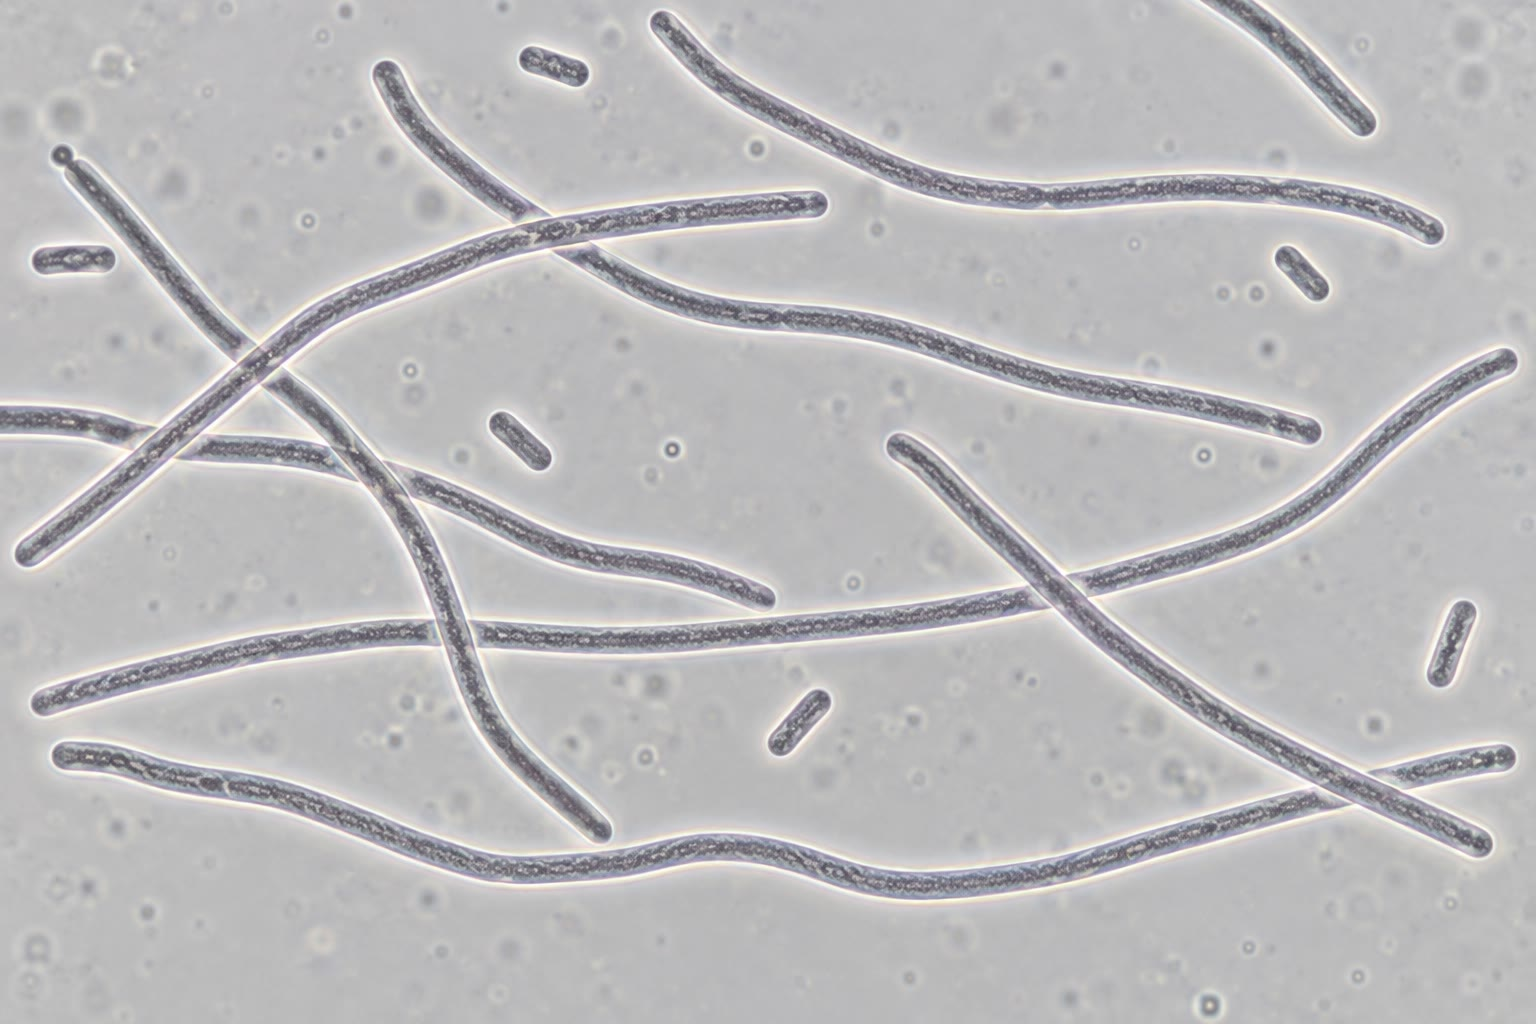
\includegraphics[width=0.46\linewidth]{images/book5/ai/b5-03-sos-filaments.jpg}\hspace{0.04\linewidth}
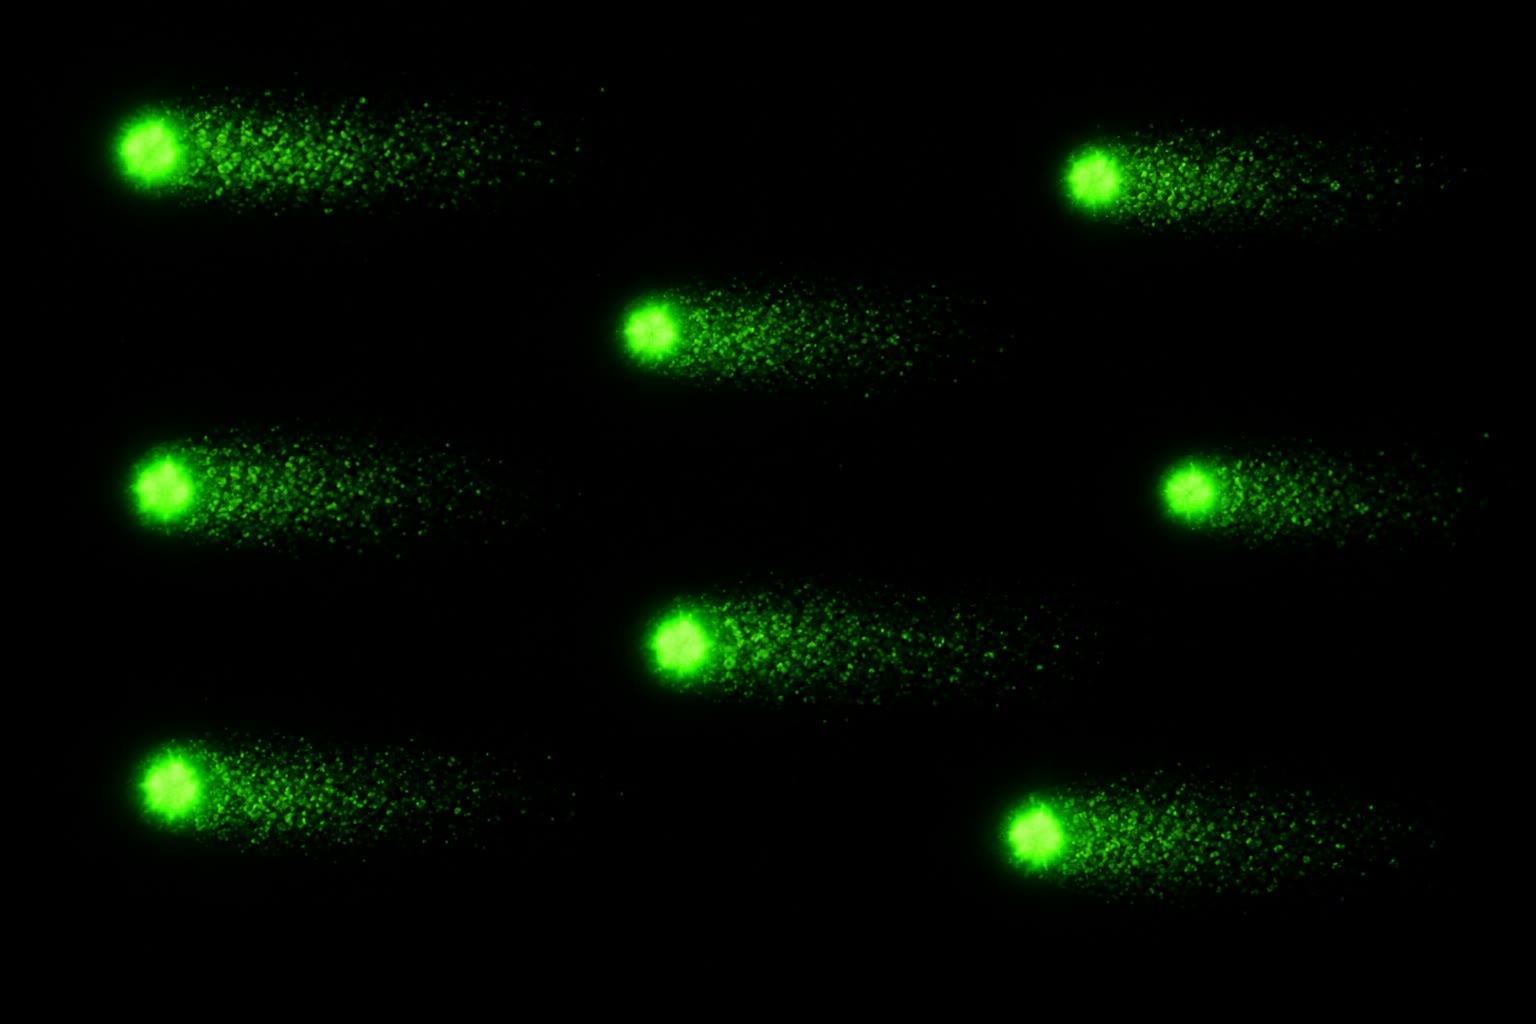
\includegraphics[width=0.46\linewidth]{images/book5/ai/b5-03-comet-assay.jpg}

{\small 左：紫外线照射后的 \emph{E.~coli}，
因 SOS 反应在 DNA 修复期间阻止细胞分裂，长成长丝。
右：彗星实验——单个细胞
包埋在凝胶中并进行电泳；断裂的 DNA 从细胞核中流出，
形成一条尾巴，尾巴的长度反映断裂的数目。}
\end{omfigure}

\begin{definition}[DNA 损伤应答]\label{def:b3:dna-repair:ddr}
\index{DNA 损伤应答}\index{ATM}\index{检查点}\index{p53}\index{γH2AX}
真核生物通过两种激酶发出\omterm{def:b3:dna-repair:lesions}{损伤}信号：\emph{ATM}，由
MRN 复合体招募到\omterm{def:b3:dna-repair:lesions}{双链断裂}处；\emph{ATR}，被招募到
停滞复制叉的单链 DNA 上。它们使数百种靶标磷酸化。
几分钟之内，\omterm{def:b3:chromatin-epigenetics:nucleosome}{组蛋白} H2AX 便发生磷酸化
（\emph{$\gamma$-H2AX}），在每个断裂周围数兆碱基范围内形成一个
灶，招募修复蛋白，并可在显微镜下计数
，每个断裂对应一个灶。激酶 Chk1 和 Chk2 使
细胞周期停止，即 \cref{ch:b3:cell-cycle-apoptosis} 中的\emph{检查点}
——其做法是使那些会推动进入 S 期或
M 期的磷酸酶失活；转录因子 \emph{p53} 经
磷酸化而稳定，诱导细胞周期蛋白依赖性激酶抑制因子 p21（使
细胞持久停滞于 G1 期）、修复基因，以及在\omterm{def:b3:dna-repair:lesions}{损伤}严重或
持续存在时，诱导杀死细胞的凋亡基因。这一应答为
修复争取时间；修复失败时，则清除细胞，而不是
让其带着破损的基因组继续分裂。
\end{definition}

\begin{omfigure}
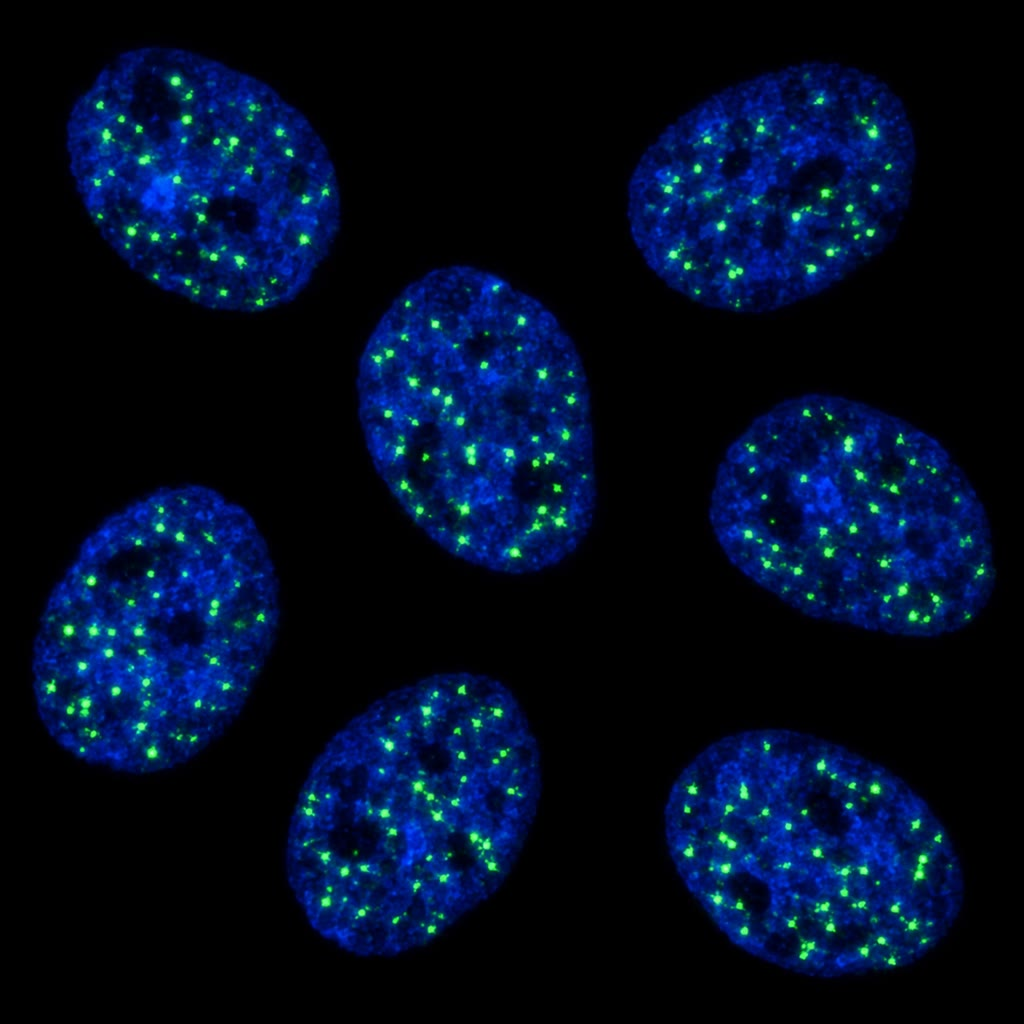
\includegraphics[width=0.4\linewidth]{images/book5/ai/b5-03-gamma-foci.jpg}

{\small 照射后一小时，细胞核（蓝色）中的 $\gamma$-H2AX 灶（绿色），
每个灶标记一个\omterm{def:b3:dna-repair:lesions}{双链断裂}；计数这些灶
可以衡量\omterm{def:b3:dna-repair:lesions}{损伤}程度，并在随后的数小时内衡量其修复情况。}
\end{omfigure}

\begin{example}[合成致死：BRCA 与 PARP]\label{ex:b3:dna-repair:parp}
遗传了一个有缺陷的 \emph{BRCA1} 或 \emph{BRCA2} 拷贝的女性，
一生中患乳腺癌的风险为 \qtyrange{50}{80}{\%}；
肿瘤发生于丢失了第二个拷贝、因而
不再能进行\omterm{def:b3:dna-repair:dsb}{同源重组}的细胞中。这类细胞
仅通过末端连接修复\omterm{def:b3:dna-repair:lesions}{双链断裂}，并积累
重排。它们还获得了一种特定的弱点。单链
断裂每天可达 \num{10000} 个，通过一条需要
酶 PARP 参与的途径修复；当 PARP 被药物抑制时，单链断裂
会持续到 S 期，在那里复制叉将每个断裂转化为
只有一端的\omterm{def:b3:dna-repair:lesions}{双链断裂}——只能通过重组修复。正常的
细胞带有一个完好的 \emph{\omterm{def:b3:dna-repair:dsb}{BRCA}} 等位基因，能够应对；肿瘤细胞则死亡。
两个单独无害的缺陷共同存在时却是致命的：该药物
通过\emph{合成致死}杀死肿瘤细胞，并保全患者的其他细胞。
\end{example}

\begin{proposition}[重组作为工具]\label{prop:b3:dna-repair:tools}
\index{位点特异性重组}\index{Cre-lox}
\omterm{prop:b3:dna-repair:tools}{位点特异性重组}酶在短的、确定的序列处切割并重新连接 DNA，
无需同源搜索或合成：噬菌体 P1 的酶
Cre 作用于 \qty{34}{bp} 的 \emph{loxP} 位点，酵母的酶 Flp 作用于
\emph{FRT} 位点。同一分子上方向相同的两个位点
会将其间的 DNA 切除成环；方向相反时则
使其倒位；位于两个分子上的位点则交换其两侧的片段。
两侧带有 \emph{loxP} 位点（称为“floxed”）的基因，只在
表达 Cre 的细胞中被删除，Cre 的启动子由实验者选定，
或在实验者选定的时间删除（若 Cre 由药物激活）。
这正是人们借以在成体肝脏或某个神经元中单独研究
一个胚胎中必需的基因的方法（见\cref{ch:b3:genetic-engineering}）。
细胞自身的\omterm{def:b3:dna-repair:dsb}{同源重组}，正是
基因打靶和 CRISPR 定向编辑借以将所选序列
写入所选位置的机制。
\end{proposition}

\begin{remark}[修复与衰老]\label{rem:b3:dna-repair:ageing}
不能修复的细胞会积累突变，衰老或死亡；
遗传性修复缺陷（Werner 综合征，缺陷在解旋酶；Cockayne 综合征，
缺陷在转录偶联修复；共济失调毛细血管扩张症，缺陷在 \omterm{def:b3:dna-repair:ddr}{ATM}）
会引起早衰的特征，正常组织的体细胞突变数
随年龄线性增长，速率约为每个细胞每年数十个
突变。积累的\omterm{def:b3:dna-repair:lesions}{损伤}是\emph{导致}
普通衰老，还是仅仅伴随衰老，尚无定论；
而修复能力是跨物种寿命的决定因素——
寿命更长的物种修复得更多——这一点已得到充分支持。
\end{remark}

\section{练习}

\begin{exercise}[$\star$]\label{exo:b3:dna-repair:1}
将下列\omterm{def:b3:dna-repair:lesions}{损伤}分为自发的或环境诱发的，并为每种\omterm{def:b3:dna-repair:lesions}{损伤}指出修复途径：
DNA 中的尿嘧啶；胸腺\omterm{def:b3:dna-repair:lesions}{嘧啶二聚体}；\omterm{def:b3:dna-repair:lesions}{8-氧代鸟嘌呤}；
复制叉后方的 G--T 错配；
G1 期的\omterm{def:b3:dna-repair:lesions}{双链断裂}。
\end{exercise}

\begin{exercise}[$\star$]\label{exo:b3:dna-repair:2}
为什么\omterm{def:b3:dna-repair:excision}{核苷酸切除修复}不需要针对每种\omterm{def:b3:dna-repair:lesions}{损伤}的专一酶，
而\omterm{def:b3:dna-repair:excision}{碱基切除修复}却需要针对每种\omterm{def:b3:dna-repair:lesions}{损伤}各有一种
糖基化酶？
\end{exercise}

\begin{exercise}[$\star$]\label{exo:b3:dna-repair:3}
叙述\omterm{prop:b3:dna-repair:fidelity}{错配修复}中的链识别问题，以及 \emph{E.~coli} 如何解决该问题。
若一个 \emph{dam} 突变体不能使任何 GATC 位点甲基化，
会出现什么情况？
\end{exercise}

\begin{exercise}[$\star$]\label{exo:b3:dna-repair:4}
一个细胞受到 \qty{2}{Gy} 的 X 射线照射，大约会产生多少个\omterm{def:b3:dna-repair:lesions}{双链断裂}？
一小时后预计可数到多少个 $\gamma$-H2AX 焦点？
为什么六小时后焦点数目更少？
\end{exercise}

\begin{exercise}[$\star\star$]\label{exo:b3:dna-repair:5}
利用\cref{prop:b3:dna-repair:fidelity}计算
每个碱基对的突变率，以及每次分裂中每个二倍体基因组产生的新突变数，
分别针对 (a) 正常细胞；(b) 缺失\omterm{prop:b3:dna-repair:fidelity}{错配修复}的细胞；
(c) 聚合酶失去外切核酸酶活性的细胞。
哪一种是更危险的突变子？
\end{exercise}

\begin{exercise}[$\star\star$]\label{exo:b3:dna-repair:6}
无碱基位点以每个细胞每天 $10^{4}$ 个的速率产生，
其修复半衰期为 \qty{15}{min}。利用\cref{thm:b3:dna-repair:load}
求细胞中无碱基位点的稳态数目。若某药物使修复速度减慢为原来的十分之一，
新的稳态数目是多少？若复制叉在 \qty{8}{h} 内复制完整个基因组，
它会遇到多少个这样的位点？
\end{exercise}

\begin{exercise}[$\star\star$]\label{exo:b3:dna-repair:7}
在 G2 期，断裂可由 NHEJ（半衰期 \qty{30}{min}）或 HR（半衰期 \qty{4}{h}）修复，两条途径均可使用。
通过 HR 途径修复的断裂占多大比例？
断裂的半衰期是多少？
然而，为什么在塌陷的复制叉处真正起作用的是 HR 途径？
\end{exercise}

\begin{exercise}[$\star\star$]\label{exo:b3:dna-repair:8}
预测下列患者的微卫星行为、肿瘤谱和对阳光的敏感性：
(a) \omterm{def:b3:dna-repair:mmr}{林奇综合征}患者；(b) \omterm{def:b3:dna-repair:excision}{着色性干皮病} A 组
患者；(c) 缺乏 Pol~$\eta$ 的
XP-V 变体患者。
\end{exercise}

\begin{exercise}[$\star\star$]\label{exo:b3:dna-repair:9}
某基因的外显子 3 两侧有两个方向相同的 \emph{loxP} 位点；
Cre 由一个仅自出生起在肝脏中活跃的启动子表达。
描述成体中肝细胞和神经元的基因型，并说明若两个位点改为方向相反，
将会发生什么。
\end{exercise}

\begin{exercise}[$\star\star\star$]\label{exo:b3:dna-repair:10}
利用 \omterm{prop:b3:dna-repair:sos}{LexA} 对其操纵基因的亲和力，
解释 SOS 反应为何先于易错聚合酶开启修复基因，
以及为何一个完全缺乏易错聚合酶的细菌，
在接受抗生素治疗的患者体内
仍可能处于劣势？
\end{exercise}

\begin{exercise}[$\star\star\star$]\label{exo:b3:dna-repair:11}
PARP 抑制剂可杀死 \emph{\omterm{def:b3:dna-repair:dsb}{BRCA}} 缺陷的肿瘤细胞，
但不杀死患者的正常细胞。请列出因果链，然后预测
肿瘤对该药物产生耐药的两种方式，
并说明如何检测每一种方式。
\end{exercise}

\begin{exercise}[$\star\star\star$]\label{exo:b3:dna-repair:12}
交叉处的基因转换产生 $3{:}1$ 的四分体。画出（或描述）一个
跨越某一标记位点、含异源双链的\omterm{def:b3:dna-repair:dsb}{霍利迪连接体}，
并说明对异源双链沿一个方向进行\omterm{prop:b3:dna-repair:fidelity}{错配修复}会得到 $3{:}1$，
沿另一方向修复则得到 $1{:}3$；若不修复，
则产生一个本身杂合的孢子（减数分裂后分离）。
为什么转换只局限于交叉点附近的标记位点？
\end{exercise}

\section{问题：一个基因组的一天}

\begin{problem}[{周末问题——计数一个人类细胞每天的损伤，将保真度阶梯相乘，
追踪一次日光照射在正常细胞和修复缺陷细胞中直至复制叉的过程，
将一次 X 射线剂量分配给两条修复途径，
并将肿瘤的弱点转化为一种药物，
最终计算复制叉遇到的二聚体数目、每个碱基的突变率，
以及被重组修复的断裂所占的
比例}]
\label{pb:b3:dna-repair:1}
数据：一个二倍体人类细胞含有 $6.4\times 10^{9}$ 个碱基对，其中 \qty{1.5}{\%}
编码蛋白质。每天的自发\omterm{def:b3:dna-repair:lesions}{损伤}：$10^{4}$ 次
\omterm{def:b3:dna-repair:lesions}{脱嘌呤}、$400$ 次胞嘧啶脱氨、$10^{4}$ 次单链
断裂。\omterm{prop:b3:dna-repair:fidelity}{保真度}：聚合酶为 $10^{-5}$，\omterm{prop:b3:dna-repair:fidelity}{校对}后留下
$10^{-2}$ 的错误，\omterm{prop:b3:dna-repair:fidelity}{错配修复}为 $10^{-3}$。一次日光浴使
每个皮肤细胞产生 $10^{5}$ 个\omterm{def:b3:dna-repair:lesions}{嘧啶二聚体}；切除修复的
半衰期通常为 \qty{2}{h}，在\omterm{def:b3:dna-repair:excision}{着色性干皮病}
中为 \qty{70}{h}；复制叉在 \qty{8}{h} 后到达；\omterm{def:b3:dna-repair:tls}{跨损伤合成}
绕过一个二聚体时产生突变的概率为 $10^{-3}$。X 射线每戈瑞
产生 $35$ 个\omterm{def:b3:dna-repair:lesions}{双链断裂}；NHEJ 半衰期为 \qty{30}{min}，HR
半衰期为 \qty{4}{h}。

\medskip
\noindent\textbf{第一部分——寻常的日子。}
\begin{enumerate}
  \item 细胞每天遭受多少次自发\omterm{def:b3:dna-repair:lesions}{损伤}，每年又遭受多少次？
        并与基因组的大小相比较。
  \item 求每次分裂中每个碱基对的突变率，
        以及每次分裂产生的新突变的期望数。
  \item 其中有多少落在蛋白质编码序列中？在从受精卵到成体皮肤细胞
        的大约 $50$ 次分裂中，
        皮肤细胞仅由复制造成的
        编码区突变有多少个？
  \item 缺乏\omterm{prop:b3:dna-repair:fidelity}{错配修复}的细胞，其突变率及
        每次分裂的突变数各为多少？一个微卫星在无\omterm{prop:b3:dna-repair:fidelity}{错配修复}时每 $10^{4}$
        次分裂滑移一次，有\omterm{prop:b3:dna-repair:fidelity}{错配修复}时每 $10^{7}$ 次分裂滑移一次。
        一个含 $10^{9}$ 个细胞的肿瘤，经 $40$ 次分裂衍生而来，
        在某一给定微卫星位点上，两种情况下分别有多少细胞
        携带滑移等位基因？（以速率 $\times$
        分裂次数 $\times$ 细胞数估算。）
  \item 胞嘧啶脱氨生成尿嘧啶，5-甲基胞嘧啶脱氨
        生成胸腺嘧啶。哪一种会被修复、由何种机制修复，哪一种会
        成为突变？请联系
        \cref{ch:b3:chromatin-epigenetics}中的 \omterm{def:b3:chromatin-epigenetics:methylation}{CpG} 缺失。
  \item 一个被氧化的鸟嘌呤（8-oxoG）在复制时与 A 配对。
        细胞具有一种糖基化酶，可识别与 C 配对的 8-oxoG，另一种
        可识别与 8-oxoG 相对的 A，还有一种水解酶能破坏被氧化的 dGTP。
        请解释各自防止的是什么，以及三者全部失效时
        会产生什么突变。
\end{enumerate}

\medskip
\noindent\textbf{第二部分——阳光下的一天。}
\begin{enumerate}[resume]
  \item 分别求正常细胞与
        XP 细胞的切除速率常数 $k$。
  \item 两种细胞中，复制叉处各残留多少个二聚体？
  \item 两种情况下，日光浴使每个细胞产生多少个突变，
        其中有多少位于编码序列中？
  \item 在童年期经历 $500$ 次此类照射后，
        两种情况下每个皮肤细胞的编码区突变数各为多少？与
        第~3~问中仅由复制造成的数目相比较。
  \item 约 $20$ 个基因，编码序列共 \qty{40}{kb}，
        一旦突变即可引发皮肤癌。求每个细胞中
        至少有一次日光浴诱发的突变落入其中之一的概率，
        在 XP 患儿中是多少？（用
        均值正确的泊松分布计算。）若有 $10^{9}$ 个受照射细胞，有多少个被击中？
  \item 解释 XP 细胞的问题为何在于复制叉，而非\omterm{def:b3:dna-repair:lesions}{损伤}本身，
        以及癌症为何只出现在皮肤中。
\end{enumerate}

\medskip
\noindent\textbf{第三部分——一次 X 射线照射。}
\begin{enumerate}[resume]
  \item 一次 \qty{2}{Gy} 剂量下，产生多少个\omterm{def:b3:dna-repair:lesions}{双链断裂}，
        若仅经 NHEJ 途径，一小时后有多少个 $\gamma$-H2AX 焦点
        （G1 期细胞）？
  \item 在 G2 期细胞中两条途径同时起作用。求
        速率常数，以及由 HR 修复的断裂所占比例。
  \item G2 期断裂的半衰期是多少？一小时后还剩多少个
        断裂？
  \item 每次 NHEJ 事件都会在连接处改变若干碱基对。若
        连接点落在编码序列中的概率为 $0.015$，且
        改变随后破坏该基因的概率为 $0.7$，
        则 \qty{2}{Gy} 剂量每个 G1 期细胞破坏多少个基因？
  \item 若有 $n$ 个同时发生的断裂，末端可能被错误连接成
        易位。设 $n(n-1)/2$ 对断裂中每一对
        被错误连接的概率为 $3\times 10^{-4}$。求
        每个细胞的易位期望数，在 \qty{2}{Gy} 与 \qty{0.2}{Gy} 下各为多少？为何
        风险随剂量的平方变化，而断裂数
        只随剂量线性变化？
  \item 同样的 \qty{2}{Gy} 剂量不是一次性瞬间给予，而是在 \qty{10}{h} 内分次给予：
        任一时刻存在多少个断裂（稳态
        ，NHEJ）？这对易位有何影响，
        以及对放射治疗分次照射的做法意味着什么？
  \item 细胞在剂量 $D$ 下的存活概率为 $e^{-D/D_{0}}$，其中
        修复完好的细胞取 $D_{0} = \qty{1.5}{Gy}$，
        缺乏 NHEJ 的细胞取 \qty{0.5}{Gy}。求
        各自在 \qty{2}{Gy} 与 \qty{6}{Gy} 下的存活率，并解释 $D_{0}$ 的含义。
\end{enumerate}

\medskip
\noindent\textbf{第四部分——肿瘤的弱点。}
\begin{enumerate}[resume]
  \item 一个 \emph{BRCA2} 缺陷的肿瘤细胞仅通过 NHEJ 修复断裂。
        利用第~14~问，求其 S/G2 期断裂中现在被不准确修复、
        而正常细胞本可准确修复的比例为多少？
        这会对其基因组在数年间产生什么影响？
  \item PARP 抑制使每日 $10^{4}$ 个单链断裂得不到修复；其中
        \qty{1}{\%} 经复制叉转化为单端
        \omterm{def:b3:dna-repair:lesions}{双链断裂}。每个细胞每天产生多少个此类断裂，
        以及为何 NHEJ 无法
        正确修复单端断裂？
  \item 解释患者的正常细胞（对
        \emph{BRCA2} 为杂合）为何能在药物作用下存活。
  \item 肿瘤通过第二次突变获得耐药性，该突变
        恢复了 \emph{BRCA2} 的阅读框。请解释，并说明
        如何检测该突变。
  \item 烷化剂化疗杀伤肿瘤细胞，
        其机制是通过\omterm{prop:b3:dna-repair:fidelity}{错配修复}：修复酶试图修复
        被烷化的碱基，并触发细胞死亡。预测该药物
        对\omterm{def:b3:dna-repair:mmr}{林奇综合征}肿瘤的作用，该肿瘤缺乏\omterm{prop:b3:dna-repair:fidelity}{错配
        修复}。
  \item 陈述三个结果：复制叉在 XP 细胞中遇到的
        二聚体数（第~8~问），正常细胞每个碱基对的突变率
        （第~2~问），以及 HR 修复的 G2 期断裂比例
        （第~14~问）。
\end{enumerate}
\end{problem}
